\documentclass[11pt]{article}

\usepackage[margin=1in]{geometry}
\usepackage[T1]{fontenc}
\usepackage[utf8]{inputenc}
\usepackage{lmodern}
\usepackage{microtype}
\usepackage{amsmath}
\usepackage{amssymb}
\usepackage{booktabs}
\usepackage{array}
\usepackage{graphicx}
\usepackage{xcolor}
\usepackage{tikz}
\usetikzlibrary{arrows.meta,positioning,fit,calc}
\usepackage{pgfplots}
\pgfplotsset{compat=1.18}
\usepgfplotslibrary{groupplots}
\usepackage{listings}
\usepackage[numbers,sort&compress]{natbib}
\usepackage{hyperref}
\usepackage{cleveref}

\hypersetup{colorlinks=true,linkcolor=blue!50!black,citecolor=green!35!black,urlcolor=blue!60!black}
\lstset{basicstyle=\ttfamily\small,columns=fullflexible,breaklines=true,frame=single,framerule=0.3pt}

\newcommand{\gofer}{Gofer}
\newcommand{\katago}{KataGo}
\newcommand{\code}[1]{\texttt{#1}}

\title{Gofer v4: A Low-Budget, Resumable Self-Play Training Pipeline\\for $9\times9$ Go, Built on the \katago{} Recipe}
\author{DevomB\\\small Gofer project}
\date{September 2026}

\begin{document}
\maketitle

\begin{abstract}
\katago{}~\citep{wu2019accelerating} showed that a handful of changes to the AlphaZero
process---playout cap randomization, global pooling, auxiliary policy, ownership and score
targets, and a growing replay window---cut the compute needed to learn Go by about
$50\times$. Even so, that result needed tens of GPUs. This report describes version~4 of the
training pipeline for \gofer{}, a small open-source Go engine. The goal is different: build
the infrastructure so a \katago{}-style run can start on free CPU runners and move to a
single rented, preemptible GPU without losing work.

Building the gate turned out to be the most valuable part. Asked to decide whether one
network was stronger than another, it could not: the answer was exactly $0.500$ every
time. Chasing that exposed eight defects, all older than this work and all invisible to
the test suite. Five were in the search. On $9\times9$ it never left the root at all,
because a stale pointer lost the flag that marks a node expanded; with that repaired,
every playout went down a single line, because first-play urgency was a flat constant no
visited child could lose to; selection maximised the \emph{opponent's} value, so more
search made the engine weaker; two passes were never treated as the end of the game; and
forced playouts, applied to every child rather than every \emph{visited} child,
outnumbered the search budget and flattened the policy training target. The other three
were in the measurement apparatus, and they are why the first five survived: the arena
drew correlated openings for one of the two roles, the reproducible strength baseline
silently enhanced both players in a way that bypassed the root, and matches stopped early
on the very statistic they were measuring. The project's own reproducible strength
baseline---200 games, identical evaluators, one side searching three times harder---had
recorded the deeper search winning \textbf{7 games in 200}, or $-576$ Elo. The same
command now returns \textbf{149 in 200}, $+186$ Elo, with the median game growing from 11
moves to 76. Every strength number the project had recorded was measuring these bugs, and
the reference baseline asserted that more search was catastrophically harmful. A later
pass over the engine, made for code quality rather than correctness, found two more of the
same kind by reading alone: a sidecar-backed gate that pointed both engines at the same
model and so returned the $0.500$ a working symmetric match would, and a transposition
table that stored no key and served colliding positions each other's evaluations.

We describe the full loop. Go self-play writes compact binary shards. A new learner masks
the policy loss to full-search positions, splits train and validation by game, augments
with the eight board symmetries, keeps an exponential moving average of the weights, and
can distill a new architecture from the current champion. An orchestrator adds sequential
(SPRT) gating, stage-level resumability, and a registry of champions that is never pruned.

Relative to the previous \gofer{} pipeline, we fix two labeling defects and a validation leak, and make the
data about $40\times$ smaller. The loop was verified end to end on CPU, with a checked
parity bound between PyTorch and ONNX Runtime. We report no playing-strength results:
no training run at scale has been done. We state precisely which \katago{} techniques we
adopt, which we change, and which are still missing, and we give the experiment protocol
that would test the claims left open.
\end{abstract}

\section{Introduction}\label{sec:intro}

AlphaGo Zero~\citep{silver2017mastering} and AlphaZero~\citep{silver2018general} learned
superhuman Go from self-play alone. They did it with enormous compute: about 41 TPU-years
for AlphaZero's main Go run, and about 74 GPU-years for the ELF OpenGo
replication~\citep{tian2019elf}, by the estimates of \citet{wu2019accelerating}.
\citeauthor{wu2019accelerating}'s \katago{} paper, the reference point throughout this
report, closed much of that gap. It surpassed ELF's final model after 19~days on fewer
than 30 V100 GPUs, a reduction of about $50\times$. It got there through a set of mostly
general techniques: playout cap randomization, policy target pruning, global pooling, an
auxiliary opponent-policy target, and auxiliary ownership and score targets.

\gofer{} is a small Go engine written in Go. It uses Chinese area scoring, MCTS with a
PUCT selection rule, a GTP interface, and ONNX neural evaluation. Its README cites
\katago{} as its inspiration. Until this work, its learning loop (``v3'') was a shell
script. The script generated self-play JSONL on a CPU cloud instance, fine-tuned a
6-block, 64-channel residual network, and promoted a candidate after an arena of up to 200 games
against the champion. Two constraints shape this report:
\begin{enumerate}
  \item \textbf{No compute budget.} The owner cannot rent a GPU today. The pipeline therefore has
        to do something useful on free CPU resources, and it has to make a future rented
        GPU, most likely a cheap preemptible instance, as productive as possible from the
        first hour.
  \item \textbf{No strength results yet.} Without a real training run, we cannot honestly claim
        that the v4 pipeline produces a stronger engine than v3, let alone one comparable to
        \katago{}. Every claim below is limited to what we measured or can derive, and
        \cref{sec:limitations} lists what remains untested.
\end{enumerate}

\paragraph{What ``better'' means here.}
The v4 pipeline improves on its predecessor in four concrete ways, and it differs from the
\katago{} paper's recipe in several deliberate ways:
\begin{itemize}
  \item \textbf{Correct targets.} v3 stored ownership in absolute colour while every other
        target is from the side to move. Its \code{policy\_opp} field held the
        \emph{previous} move's policy rather than the opponent's reply. It split
        validation by row, so near-identical positions from one game landed on both sides
        of the split. All three are fixed, and tests cover each fix
        (\cref{sec:selfplay,sec:learner}).
  \item \textbf{Adoption of \katago{}'s general techniques at small scale.} We adopt
        playout-cap-aware training, global-pooling bias blocks, the auxiliary
        opponent-policy head, ownership and score heads, and the power-law replay window
        (\cref{sec:learner,sec:orchestration}). One change is deliberate:
        \katago{} \emph{discards} fast-search positions, while we keep them and mask only
        the policy loss. \Cref{sec:learner-masking} discusses the correlation risk this
        brings.
  \item \textbf{Cheaper iteration.} The data is about $40\times$ smaller, with no JSON
        parsing (\cref{sec:selfplay}), and self-play for the next cycle overlaps training.
  \item \textbf{Controlled promotion errors.} Gating uses a sequential probability ratio
        test~\citep{wald1945sequential}. It stops early on clearly worse or clearly better
        candidates, and it cuts the false-promotion rate at zero true gain from 8.0\% for
        v3 to 2.4\%, while promoting a $+50$ Elo candidate 90\% of the time against v3's
        67\%. The price is \emph{longer} gates near zero gain
        (\cref{sec:orchestration}), so this is an error-control gain, not a cost saving.
  \item \textbf{Eight defects, found by building the gate.} Five in the search: a stale
        pointer that stopped it leaving the root on $9\times9$; a first-play-urgency
        constant that collapsed the visit distribution---the policy training target---onto
        one move; forced playouts that outnumbered the search budget and flattened the same
        target; an inverted value sign that made more search strictly weaker; and a search
        that never saw a game end. Three in the measurement apparatus, which is why the
        others survived: correlated per-game seeds, a strength baseline that silently
        enhanced both players, and matches that stopped on the statistic under test. On the project's own
        reproducible baseline, the side searching three times harder went from 7 wins in
        200 games to 136, a sign flip from $-576$ to $+131$ Elo
        (\cref{sec:pipeline-found}). This is the strongest argument in this report
        for building the measurement apparatus before spending money on compute.
  \item \textbf{Robustness to cheap hardware.} Every stage can resume after a crash or
        preemption, the trainer can continue mid-run, and champions are immutable and
        never pruned (\cref{sec:orchestration,sec:infra}). A distillation path lets the
        project change network architecture without discarding the champion's knowledge
        (\cref{sec:learner-distill}). That cost was the reason an earlier ablation kept the
        6$\times$64 network.
\end{itemize}

\paragraph{Contributions.}
(i)~A complete, tested description of a small-scale \katago{}-style pipeline for
$9\times9$ Go, from Go self-play to a gated, published ONNX champion. (ii)~An explicit
technique-by-technique comparison with \citet{wu2019accelerating}
(\cref{tab:overview-compare}). (iii)~Measurements of what can be measured without a
training run: data size, load time, parameter and compute budgets, CPU inference latency,
export parity, exact gate operating characteristics, and end-to-end cycle timings
(\cref{sec:eval}), together with the engine defects that apparatus exposed
(\cref{sec:pipeline-found}).
(iv)~An ablation protocol, modelled on \katago{}'s, for the experiments that would settle
the open questions (\cref{sec:conclusion}).

\paragraph{Organisation.}
\Cref{sec:background} reviews AlphaZero-style training and the relevant parts of
\katago{}. \Cref{sec:overview} gives the system overview and comparison tables.
\Cref{sec:selfplay,sec:learner,sec:orchestration,sec:infra} describe self-play data, the
learner, orchestration, and infrastructure in turn. \Cref{sec:eval} reports measurements,
\cref{sec:limitations} lists limitations, and \cref{sec:conclusion} concludes.

\section{Background}\label{sec:background}

\subsection{AlphaZero-style self-play}

Monte Carlo tree search~\citep{coulom2006efficient,kocsis2006bandit} guided by a policy
and value network is the basis of AlphaGo~\citep{silver2016mastering}, AlphaGo
Zero~\citep{silver2017mastering}, and AlphaZero~\citep{silver2018general}, together with
their open reproductions ELF OpenGo~\citep{tian2019elf}, Leela
Zero~\citep{pascutto2019leela} and SAI~\citep{morandin2019sai}.

Each playout descends from the root. At each node it picks the child $c$ that maximises
the PUCT score~\citep{rosin2011multi,silver2017mastering}:
\begin{equation}
  \mathrm{PUCT}(c) = V(c) + c_{\mathrm{PUCT}}\,P(c)\,\frac{\sqrt{\sum_{c'} N(c')}}{1 + N(c)},
  \label{eq:puct}
\end{equation}
where $V$ is the mean value of the subtree, $P$ the network's prior and $N$ the visit
count. The root visit distribution $\pi$ becomes the policy target, the game outcome $z$
the value target, and the network is trained to minimise
\begin{equation}
  L = (z - \hat v)^2 - \textstyle\sum_m \pi(m)\log\hat\pi(m) + c\,\lVert\theta\rVert^2 .
  \label{eq:az-loss}
\end{equation}
AlphaGo Zero also exploited the eight rotations and reflections of the board to augment
its training data~\citep{silver2017mastering,silver2018general}, and it gated each new
network by requiring a 55\% win rate against the current one over 400
games~\citep{silver2017mastering}. AlphaZero dropped gating and trained
continuously~\citep{silver2018general}.

\subsection{The \katago{} recipe}\label{sec:bg-katago}

\citet{wu2019accelerating} keeps the AlphaZero skeleton and changes the parts listed
below. This report refers back to them by name.
\begin{description}
  \item[Playout cap randomization.] Only a fraction $p=0.25$ of turns gets a full search
    (a cap of $N$ nodes); the rest use a fast search with cap $n<N$. Early in the run
    $(N,n)=(600,100)$, rising to $(1000,200)$. \emph{Only full-search turns are recorded
    for training}. Fast turns exist to generate more games, and therefore more value
    targets, per unit of compute. Informal evidence from Leela Zero suggests that policy
    learning needs far more playouts per move than value learning~\citep{forsten2019optimal}.
  \item[Forced playouts and policy target pruning.] Children of the root get a minimum
    number of playouts, $n_{\mathrm{forced}}(c)=(k P(c)\sum N)^{1/2}$ with $k=2$. The
    forced extras are then subtracted from the policy target, so exploration no longer
    pollutes what the policy learns.
  \item[Global pooling.] Pooling layers compute each channel's mean, its mean scaled by board
    width, and its maximum. A fully connected layer maps these to a per-channel bias for
    another set of channels. The structure follows the first convolution of some residual
    blocks and appears in the policy and value heads. It is related to
    Squeeze-and-Excitation~\citep{hu2018squeeze}.
  \item[Auxiliary policy target.] The policy head also predicts the opponent's reply, with
    weight $w_{\mathrm{opp}}=0.15$~\citep{tian2016better}.
  \item[Ownership and score targets.] The network predicts the final owner of each point
    (cross-entropy with $w_o = 1.5/b^2$) and the final score, via a ``pdf'' and a ``cdf''
    loss each with weight $0.02$. This follows the multi-labelled value networks of
    \citet{wu2018multilabelled}.
  \item[Game-specific input features.] Liberties, ladders, pass-alive regions and komi
    parity.
  \item[Training details.] SGD with momentum 0.9, batch 256, $c_{L2}=3\times10^{-5}$,
    value-loss scale $c_g=1.5$. The per-sample learning rate is fixed, lowered for the
    first 5M samples and near the end. Samples are drawn uniformly from a moving window
    whose size grows sublinearly with the total amount of data:
    \begin{equation}
      N_{\mathrm{window}} = c\left(1 + \beta\,\frac{(N_{\mathrm{total}}/c)^{\alpha} - 1}{\alpha}\right),
      \quad c=250{,}000,\ \alpha=0.75,\ \beta=0.4
      \label{eq:window}
    \end{equation}
    \citep[App.~C]{wu2019accelerating}. Candidates are an exponential moving average of
    weight snapshots, in the spirit of stochastic weight
    averaging~\citep{izmailov2018averaging}. A candidate must win at least 100 of 200 games
    to replace the current network~\citep[App.~E]{wu2019accelerating}.
\end{description}
\citeauthor{wu2019accelerating}'s ablations (Table~2 of that paper) put the training-time
factor of each technique between $1.25\times$ and $1.65\times$ at about two days of
compute. The factors multiply to roughly $9\times$. This report uses those factors only as
motivation. We do not reproduce them.

\subsection{\gofer{} before this work}\label{sec:bg-gofer}

\gofer{} plays under Chinese area scoring with Tromp--Taylor-style
evaluation~\citep{tromp2014go}. Its network interface is fixed by a feature schema:
\begin{itemize}
  \item \textbf{Spatial input} ($8\times S\times S$): own stones, opponent stones, empty
        points, the simple-ko point, a to-move plane, and the last three moves.
  \item \textbf{Global input} (4 values): komi$/10$, the normalised move number, and one-hot
        side to move.
  \item \textbf{Outputs}: $S^2+1$ policy logits (pass last) and a scalar $\tanh$ value from the
        side to move's perspective.
\end{itemize}

Search uses \cref{eq:puct} with $c_{\mathrm{PUCT}}=1.1$. Unvisited children get a fixed
value of $-0.2$, whereas \katago{}'s first-play urgency is the parent value minus
$0.2\sqrt{P_{\mathrm{explored}}}$. In self-play, root Dirichlet noise ($\alpha=0.15$, blend $0.25$) is applied on
every move, fast and full, whereas \katago{} disables it on fast searches. Full searches
also force a minimum number of visits on each root child ($2 + \lfloor\sqrt{P(c)(N+1)}\rfloor$
for playout cap $N$, versus \katago{}'s $\sqrt{2P(c)\sum N}$), and they prune the policy
target by dropping children with fewer than two visits (\cref{sec:selfplay-search}). Inference runs through ONNX
Runtime~\citep{onnxruntime2021}, either in-process or through a Python sidecar.

The v3 loop, documented in the repository's ADR~0003, ran the following cycle:
\begin{enumerate}
  \item Self-play: 200 games per cycle, 200 playouts per move with playout cap randomization
        ($p=0.20$, fast cap 50), keeping only full-search rows.
  \item Replay: append the games to a JSONL replay file capped first-in-first-out at 50{,}000
        rows.
  \item Training: fine-tune the champion's 6-block, 64-channel network (``6$\times$64'') for
        15 epochs with SGD.
  \item Gating: export the candidate to ONNX and play up to 200 arena games against the
        champion. Promote if it scores at least 0.55 with the lower Wilson
        bound~\citep{wilson1927probable} above 0.5. The arena stops early: after 20 games
        once 0.55 is out of reach, and after 100 games once the promotion condition holds.
\end{enumerate}

ADR~0005 compared net sizes offline and found a thin validation-loss edge for a 4$\times$48
network. It kept 6$\times$64 anyway, because changing architecture breaks warm-starting and
was estimated to cost 4--5 days and about 20 cycles to recover the champion's strength on
the project's CPU instance. \Cref{sec:learner-distill} targets exactly that cost.

\section{System Overview}\label{sec:overview}

\Cref{fig:overview-loop} shows one v4 cycle. Generation $k$ is the current champion,
stored as immutable ONNX, PyTorch and checkpoint files. It plays self-play games in the Go
engine, which writes one compressed shard per cycle (\cref{sec:selfplay}). The learner
warm-starts from generation $k$'s weights and trains on a window over all shards
(\cref{sec:learner}). It then exports a candidate, and that export must pass a numeric
parity check. The orchestrator gates the candidate against generation $k$ with a
sequential test. If it passes, the candidate becomes generation $k{+}1$ and is published
to a champion registry (\cref{sec:orchestration}). Meanwhile, self-play for the next cycle
is already running.

\begin{figure}[htbp]
\centering
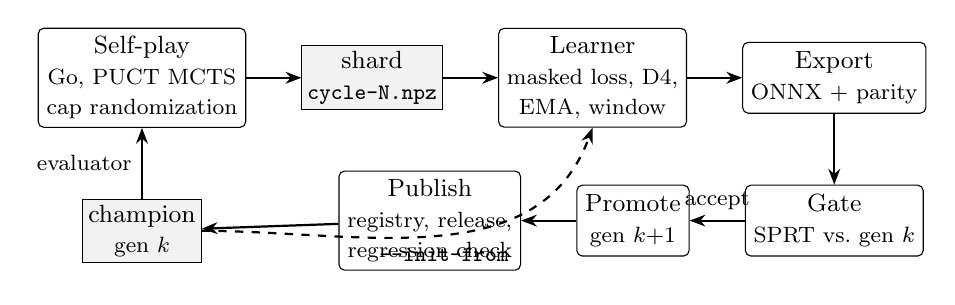
\begin{tikzpicture}[
  node distance=5mm and 7mm,
  box/.style={draw, rounded corners=2pt, align=center, font=\small, minimum height=9mm, inner sep=3pt},
  data/.style={draw, align=center, font=\small, minimum height=7mm, inner sep=2pt, fill=gray!10},
  arr/.style={-{Stealth[length=2mm]}, thick},
]
\node[box] (sp) {Self-play\\\footnotesize Go, PUCT MCTS\\\footnotesize cap randomization};
\node[data, right=of sp] (sh) {shard\\\footnotesize\code{cycle-N.npz}};
\node[box, right=of sh] (tr) {Learner\\\footnotesize masked loss, D4,\\\footnotesize EMA, window};
\node[box, right=of tr] (ex) {Export\\\footnotesize ONNX + parity};
\node[box, below=9mm of ex] (ga) {Gate\\\footnotesize SPRT vs.\ gen $k$};
\node[box, left=of ga] (pr) {Promote\\\footnotesize gen $k{+}1$};
\node[box, left=of pr] (pu) {Publish\\\footnotesize registry, release,\\\footnotesize regression check};
\node[data, below=9mm of sp] (ch) {champion\\\footnotesize gen $k$};
\draw[arr] (sp) -- (sh);
\draw[arr] (sh) -- (tr);
\draw[arr] (tr) -- (ex);
\draw[arr] (ex) -- (ga);
\draw[arr] (ga) -- node[above, font=\footnotesize]{accept} (pr);
\draw[arr] (pr) -- (pu);
\draw[arr] (pu) -- (ch);
\draw[arr] (ch) -- node[left, font=\footnotesize]{evaluator} (sp);
\draw[arr, dashed] (ch.east) to[out=0, in=250] node[below right, font=\footnotesize, pos=0.35]{\code{--init-from}} (tr.south);
\end{tikzpicture}
\caption{One v4 training cycle. Every arrow is a resumable stage recorded in the run's
state file. Self-play for cycle $N{+}1$ starts while cycle $N$ trains and gates.}
\label{fig:overview-loop}
\end{figure}

\paragraph{Interfaces.}
The three components meet at two narrow contracts. That let two developers (here, two
agent sessions) build them in parallel and test them separately.
\begin{enumerate}
  \item \textbf{Data.} GOFER SHARD v1 is a \code{.npz} archive with a fixed set of typed
        arrays (\cref{tab:selfplay-shard} in \cref{sec:selfplay}). The Go engine writes
        it, and the learner's packer can also produce it from legacy JSONL.
  \item \textbf{Learner command line.} The trainer takes \code{--data} (files or directories),
        \code{--window-rows}, \code{--init-from} or \code{--continue}, and an optional
        \code{--config} preset. It writes \code{best.pt}, a self-describing
        \code{best.ckpt}, a full-state \code{last.pt}, and a \code{summary.json} with
        fixed keys. The exporter takes a checkpoint and writes an ONNX file whose input and
        output names match the engine's schema, exiting non-zero if parity fails.
\end{enumerate}

\paragraph{Comparison.}
\Cref{tab:overview-compare} places v4 next to the v3 loop and the published \katago{}
recipe~\citep{wu2019accelerating}, one technique per row. Four symbols are used:
\checkmark{} means adopted as published, $\sim$ means adopted with a stated change,
\texttimes{} means absent, and ``new'' means not in the \katago{} paper.

\begin{table}[htbp]
\centering
\footnotesize
\begin{tabular}{@{}>{\raggedright\arraybackslash}p{3.9cm}>{\raggedright\arraybackslash}p{3.0cm}>{\raggedright\arraybackslash}p{2.6cm}>{\raggedright\arraybackslash}p{5.5cm}@{}}
\toprule
Technique & \katago{} paper & \gofer{} v3 & \gofer{} v4 \\
\midrule
Playout cap randomization & $p{=}0.25$, fast turns discarded & $p{=}0.20$, discarded & $\sim$ $p{=}0.20$; fast turns kept, policy loss masked (\S\ref{sec:learner-masking}) \\
Forced playouts + target pruning & \checkmark & $\sim$ simplified & $\sim$ unchanged: forced root visits; children with ${<}2$ visits dropped from target (\S\ref{sec:selfplay-search}) \\
Global pooling bias & \checkmark{} (mean, scaled mean, max) & \texttimes & $\sim$ mean + max; \code{gpool} nets only \\
Auxiliary opponent policy & \checkmark{} $w{=}0.15$ & \texttimes{} (label wrong) & \checkmark{} $w{=}0.15$, \code{gpool} nets \\
Ownership target & \checkmark{} cross-entropy & $\sim$ MSE, absolute frame & $\sim$ MSE on $\tanh$, side-to-move frame \\
Score target & pdf + cdf losses & \texttimes & $\sim$ Huber on margin$/20$ \\
Go-specific input features & liberties, ladders, \dots & \texttimes & \texttimes{} (schema v2 unchanged) \\
Rules / board-size randomization & \checkmark & \texttimes & \texttimes{} (net is size-agnostic) \\
Symmetry augmentation & --- & \texttimes & new: per-sample D4 \\
Replay window & power law, eq.~\eqref{eq:window} & FIFO 50k rows & \checkmark{} power law + recency weighting \\
Validation split & --- & by row (leaks) & new: by game \\
Weight averaging & EMA of snapshots & \texttimes & $\sim$ per-step EMA, $0.999$ \\
LR schedule & fixed, reduced early/late & constant & $\sim$ warmup + cosine per cycle \\
Architecture change & train next size in parallel & re-bootstrap & new: distillation from champion \\
Gating & ${\ge}100/200$ wins & 0.55 + Wilson, ${\le}200$ games, interim stops & new: SPRT + Wilson fallback; fewer false promotions \\
Preemption safety & --- & restart cycle & new: stage + step resume \\
Data format & --- & JSONL & new: binary shards, ${\sim}40\times$ smaller \\
\bottomrule
\end{tabular}
\caption{Technique-by-technique comparison. ``---'' means the \katago{} paper does not
describe the item. The v4 column covers only what is implemented and tested. None of the
v4 differences has been tested for playing strength (\cref{sec:limitations}).}
\label{tab:overview-compare}
\end{table}

The table is deliberately balanced. On the core learning techniques, v4 is a
\emph{subset} of \katago{} with a few simplifications. Policy target pruning is only a
visit-threshold approximation, and the score-belief distribution, Go-specific features
and rules randomization are all missing. The additions
are mostly engineering: data format, resumability, sequential gating, distillation. These
matter when compute is scarce and preemptible. They do not change what the network can
learn in principle.

\section{Self-Play and the Training Data}
\label{sec:selfplay}

Self-play runs in the Go engine, which is written in Go~\citep{donovan2015go}. This
section covers how a game is played, what each position is labelled with, and the binary
\emph{shard} format that replaces JSONL between the engine and the learner.

\subsection{Search during self-play}
\label{sec:selfplay-search}

Each move is chosen by Monte Carlo tree search with the PUCT selection rule of
\cref{eq:puct}~\citep{rosin2011multi,silver2017mastering}, using $c_{\mathrm{PUCT}}=1.1$
as in \citet{wu2019accelerating}. Two details differ from \katago{}. An unvisited child is
given the fixed value $-0.2$, whereas \katago{}'s first-play urgency is the parent's value
minus $0.2\sqrt{P_{\mathrm{explored}}}$. And the constant $1.03$, which \katago{} and
SAI~\citep{morandin2019sai} use as a softmax temperature on the root policy, is applied
in \gofer{} as a divisor on the root children's mean values. Root priors are mixed with Dirichlet noise ($\alpha=0.15$, weight $0.25$) on \emph{every}
self-play move. \katago{} instead turns noise and other exploration off on fast searches
to keep them as strong as possible~\citep[\S3.1]{wu2019accelerating}.

\paragraph{Playout cap randomization.}
Following \citet[\S3.1]{wu2019accelerating}, each move is a \emph{full} search (cap $N$)
with probability $p$, and otherwise a \emph{fast} search (cap $n<N$). The \gofer{}
defaults are $p=0.20$, $N=200$ and $n=50$; \katago{}'s main run used $p=0.25$ and
$(N,n)=(600,100)$, later raised to $(1000,200)$. The configurations in
\cref{sec:infra} change these values per deployment.

\paragraph{Forced playouts and target pruning (simplified).}
Full searches force a minimum number of visits to every root child $c$ that has been
expanded:
\begin{equation}
  n_{\mathrm{forced}}(c) = k + \left\lfloor \sqrt{P(c)\,(N+1)} \right\rfloor, \qquad k = 2,
  \label{eq:gofer-forced}
\end{equation}
where $P(c)$ is the noised prior. \katago{} uses
$n_{\mathrm{forced}}(c)=\bigl(kP(c)\sum_{c'}N(c')\bigr)^{1/2}$ and forces these visits by
setting the urgency of an under-visited child to infinity inside the search. \gofer{}
instead runs the forced playouts as a separate pass, right after the root is expanded and
before the main search.
The policy target differs more. \katago{} subtracts forced visits from each child only as
long as that child would not have overtaken the best child under PUCT. \gofer{} simply
removes children with fewer than two visits and renormalizes. This is cruder: it removes
single-visit noise but keeps any extra visits that forcing added to a child that stayed
bad. Both mechanisms predate v4 and are unchanged by it.

\paragraph{Two corrections to the search.}
Validating the v4 gate uncovered two defects in this search, both predating v4.
Selection used a child's mean without negating it, although node values are kept
from each node's own side to move, so the engine was choosing the move best for
its opponent; and two consecutive passes were not treated as the end of the
game, so a finished position was scored by the evaluator rather than by the
rules. \Cref{sec:pipeline-found} gives the evidence and the measured effect.
Everything described in this section is the corrected search.

\paragraph{Move selection and parallelism.}
For the first 16 plies the move is sampled in proportion to visit counts ($\tau=1$); after
that the most-visited move is played. The policy target is always the full visit
distribution, whatever move is played. Games run concurrently and share one batched
evaluator, so the neural network sees real batches. Each game's random generator is seeded
from the run seed and the game index only, so the output does not depend on how many games
run in parallel. It can still depend on the inference backend if two backends return
different network outputs; in our runs the two backends produced identical row counts
from the same seeds (\cref{sec:pipeline-eval}). Seeds are derived by mixing the run seed
with the game index rather than by adding them: consecutive seeds draw correlated
openings, which costs game diversity here and, in the arena, biased results outright
(\cref{sec:pipeline-found}).

\subsection{Labels and a common frame}
\label{sec:selfplay-labels}

Each recorded position gets the 8 binary input planes and 4 global features of
\cref{sec:learner-data}, plus these targets:
\begin{itemize}
  \item $\pi$: the root visit distribution over the $S^2+1$ moves (pass is the last entry);
  \item $z \in \{-1,0,+1\}$: the game result;
  \item $s$: the final area-score margin, with komi included;
  \item $o \in \{-1,0,+1\}^{S^2}$: the final owner of each point;
  \item $\pi_{\mathrm{opp}}$: the policy target of the \emph{next} ply, i.e.\ the
        opponent's reply, as in \citet{tian2016better} and \citet[\S3.4]{wu2019accelerating};
  \item a flag saying whether the move was a full search.
\end{itemize}
In v4, every target is expressed from the side to move, the same frame as the
``own/opponent'' input planes. Under area scoring every point belongs to one player or to
neither, so each row satisfies an exact identity:
\begin{equation}
  s \;=\; \sum_{i=1}^{S^2} o_i \;-\; \kappa\,\sigma, \qquad
  \sigma = \begin{cases} +1 & \text{Black to move}\\ -1 & \text{White to move}\end{cases}
  \label{eq:score-identity}
\end{equation}
Here $\kappa$ is the komi, which goes to White. The shard writer's test checks
\cref{eq:score-identity} on every row of real self-play output, and the fixture shard
shared with the learner's tests satisfies it with zero error.

\paragraph{Two defects in the v3 labels.}
Comparing the v3 JSONL fields with this frame found two errors. Neither raised an
exception, and both went unnoticed in v3.
\begin{enumerate}
  \item \textbf{Ownership frame.} v3 wrote ownership in the absolute frame (Black $=+1$)
        for every row, while value and the input planes are side-to-move. For
        White-to-move rows the target pointed the wrong way: the network had to recover
        the colour from the side-to-move plane just to learn a sign flip.
  \item \textbf{Opponent policy.} The field named \code{policy\_opp} held the policy of
        the \emph{previous} ply, not the opponent's reply. It is correlated with the
        right target, which is why nothing looked wrong. But the auxiliary loss it was
        meant to feed would have taught the network to predict the past.
\end{enumerate}
v4 fixes both in the engine. The shard format
stores the side-to-move ownership and the true next-ply policy. The JSONL writer keeps
its old field meanings for compatibility and adds \code{policy\_next} and
\code{score\_margin}; the learner corrects legacy rows when it loads them
(\cref{sec:learner-data}). $\pi_{\mathrm{opp}}$ is recorded only when the next ply was a
full search. After a fast search the visit distribution is too noisy to imitate, and the
row stores an all-zero vector, which the loss treats as missing.

\paragraph{Keeping fast-search rows.}
\katago{} records only full-search positions~\citep[\S3.1]{wu2019accelerating}, and v3 did
the same (\code{-full-only}). v4 shards keep every position and flag fast ones with
$\code{full\_search}=0$. The learner then masks the two policy losses to full-search rows
and trains value, ownership and score on every row (\cref{sec:learner-masking}). With
$p=0.2$ this gives about $5\times$ more rows per game for those heads, at no extra
self-play cost. The benefit is smaller than that ratio suggests. \citet{wu2019accelerating}
note that value training is limited by the number of \emph{games}, since there is one
noisy result per game. Extra positions from the same game share the same $z$ and are
strongly correlated. The gain we expect is therefore mostly in the per-point ownership
signal and in the variety of positions seen, not in independent value labels. The risk
is overfitting to game outcomes. The learner's game-level validation split
(\cref{sec:learner-data}) is what would reveal it. This choice has not been ablated for
strength (\cref{sec:limitations}).

\subsection{The shard format}
\label{sec:selfplay-shards}

When the output path ends in \code{.npz}, the engine writes a \emph{Gofer shard v1}. This
is a standard NumPy archive~\citep{harris2020array}: a ZIP file~\citep{pkware2022zip} of
\code{.npy} arrays~\citep{kern2007npy}, compressed with DEFLATE~\citep{deutsch1996deflate}.
There is one shard per self-play run, and every row in a shard has the same board size.
\Cref{tab:selfplay-shard} lists the arrays. Any \code{np.load} can read a shard, so the
learner, the replay index and ad-hoc analysis all use it without a custom parser. The
learner's JSONL packer produces the same layout, so the two producers are
interchangeable.

\begin{table}[htbp]
\centering
\small
\begin{tabular}{@{}llll@{}}
\toprule
Array & dtype & Shape & Content \\
\midrule
\code{spatial}      & uint8   & $[R,8,S,S]$ & binary input planes \\
\code{globals}      & float32 & $[R,4]$     & komi$/10$, move$/(S^2{+}1)$, is-black, is-white \\
\code{policy}       & float32 & $[R,S^2{+}1]$ & $\pi$, root visit distribution \\
\code{policy\_opp}  & float32 & $[R,S^2{+}1]$ & $\pi_{\mathrm{opp}}$, next-ply target (zeros if absent) \\
\code{value}        & float32 & $[R]$       & $z$, side to move \\
\code{score}        & float32 & $[R]$       & $s$, side to move, komi included \\
\code{ownership}    & int8    & $[R,S^2]$   & $o$, side to move \\
\code{full\_search} & uint8   & $[R]$       & 1 if the move was a full search \\
\code{game\_id}     & int32   & $[R]$       & game index within the shard \\
\code{move\_num}    & int16   & $[R]$       & ply number \\
\code{meta}         & uint8   & $[K]$       & UTF-8 JSON: format, version, board size, rows, games, \\
                    &         &             & komi, seed, generating model (ONNX hash), commit \\
\bottomrule
\end{tabular}
\caption{Arrays in a Gofer shard v1 with $R$ rows on an $S\times S$ board. Every target
uses the side-to-move frame.}
\label{tab:selfplay-shard}
\end{table}

Three properties matter for the rest of the pipeline:
\begin{itemize}
  \item \emph{Atomic writes.} The engine writes to a temporary file and renames it at the
        end, so a crash never leaves a truncated shard for the trainer to read.
  \item \emph{Immutability.} No later stage rewrites a shard, so the replay buffer is just a
        choice of which shards to read (\cref{sec:orch-replay}), and copying a run
        directory between machines is incremental.
  \item \emph{Provenance.} The \code{meta} array records which network generated the games
        (the first 8 bytes of its ONNX SHA-256, or \code{heuristic}). The orchestrator can
        read it without decompressing any data array.
\end{itemize}

\paragraph{Size.}
We measured size on the same four self-play games (seed 1, 20 playouts, 327 positions)
written in both formats. JSONL~\citep{bray2017json} took 779{,}565 bytes (2{,}384 bytes per
row), and the shard took 18{,}969 bytes (58 bytes per row), $41\times$ smaller.
Uncompressed, a shard row is 1{,}416 bytes, dominated by the 648 bytes of input planes and
the two 328-byte policy vectors. DEFLATE does the rest: the planes are binary and sparse,
and most policy entries are exactly zero. The learner's packer, run on a larger legacy file
(\cref{sec:eval}), gives a similar $38\times$. Loading a shard is one decompression per
array, with no per-number text parsing.

\section{The Learner}\label{sec:learner}

The learner is the Python package \code{gofer\_train}, built on
PyTorch~\citep{paszke2019pytorch}. It reads shards, trains one candidate per cycle, and
exports it. The v3 command-line tools keep their names and flags and now call into it.

\subsection{Data path}\label{sec:learner-data}

\paragraph{Loading.}
A source may be a legacy JSONL file, one shard, or a directory of shards. Directories are
ordered oldest to newest by modification time. Given a window of $W$ rows (from the
orchestrator, eq.~\eqref{eq:window}), the loader walks the sources from newest to oldest,
stops once $W$ rows are collected, and keeps exactly the newest $W$. Old shards are never
decompressed. Game identifiers are re-based per source, so games stay distinct across
shards.

\paragraph{Legacy JSONL.}
Old data is converted into shard conventions on load:
\begin{itemize}
  \item Ownership, stored with Black $=+1$, is multiplied by $-1$ on White-to-move rows.
  \item The field named \code{policy\_opp} is dropped, because in v3 it held the policy of
        the move \emph{before} the current position. The correct reply target
        \code{policy\_next}, added to JSONL in v4, is used when present.
  \item Game boundaries are recovered from resets of the move number, since v3 recorded
        no game id.
\end{itemize}
A test compares converted ownership with the raw file for every row.

\paragraph{Device residency.}
The window fits comfortably in accelerator memory. 50{,}000 $9\times9$ rows take
$50{,}000\times8\times81$ bytes $\approx$ 32\,MB of \code{uint8} planes, plus float
targets. So the whole window is copied to the training device once. Each step gathers a
batch by index on the device and converts planes to float there. This removes the v3
\code{DataLoader}, which built a tensor from a Python list for every row, every epoch, and
it removes host-to-device copies from the inner loop.

\paragraph{Game-level split.}
Positions from one game are strongly correlated.
\citet{silver2016mastering} sampled one position per game for exactly this reason when
training AlphaGo's value network. v3 split train and validation by row, so a validation
position usually had near-duplicates in training, and validation loss partly measured
memorisation. v4 assigns whole games to one side. A test checks that the two sets of game
ids are disjoint. One consequence: v4 validation losses are \emph{not comparable} with v3
numbers.

\paragraph{Recency sampling.}
With the default decay $\lambda=0$, batches are drawn uniformly from the window, as in
\katago{}. With $\lambda>0$, row $i$ of an $n$-row window (0 = oldest) is drawn with
probability proportional to $\exp(\lambda(i/n-1))$, so the newest data is sampled
$e^{\lambda}$ times as often as the oldest. \katago{} does not use this. It is offered as
a knob for small runs where the window is dominated by early, weaker games. The CPU preset
uses $\lambda=1.5$ and the GPU preset $\lambda=2$. Neither value has been tuned.

\paragraph{Symmetry augmentation.}
Each sample in a batch gets an independent random element of the dihedral group $D_4$.
The same element is applied to the spatial planes (all are point-local, including ko and
move history), to the $S^2$ board entries of both policy targets (the pass entry is left
alone), and to the ownership map. A test places one asymmetric stone together with its
policy mass and ownership, and checks two things: under all sampled symmetries the three
stay on the same point, and all eight images of the point are reached.

\subsection{Loss}\label{sec:learner-loss}\label{sec:learner-masking}

Let a batch $B$ have rows $i$ with full-search flag $f_i$, value target $z_i\in\{-1,0,1\}$,
policy target $\pi_i$, reply target $\pi^{\mathrm{opp}}_i$ (possibly empty), ownership
$o_i\in\{-1,0,1\}^{S^2}$ and final margin $s_i$ (possibly unknown). All targets are from
the side to move. Define the row sets
\begin{equation*}
  F = \{i : f_i = 1,\ \textstyle\sum\pi_i > 0\},\quad
  F^{\mathrm{opp}} = \{i : f_i = 1,\ \textstyle\sum\pi^{\mathrm{opp}}_i > 0\},\quad
  K = \{i : s_i \text{ known}\}.
\end{equation*}
With $\mathrm{CE}(p,q) = -\sum_m p(m)\log q(m)$ and $\mathrm{mean}_X$ the mean over a set
$X$ (zero if $X$ is empty), the loss is
\begin{align}
  L ={}& w_p\,\mathrm{mean}_{F}\,\mathrm{CE}(\pi_i,\hat\pi_i)
       + w_v\,\mathrm{mean}_{B}\,(z_i-\hat v_i)^2
       + w_o\,\mathrm{mean}_{B}\,\tfrac{1}{S^2}\lVert o_i-\hat o_i\rVert^2 \nonumber\\
      &+ w_{\mathrm{opp}}\,\mathrm{mean}_{F^{\mathrm{opp}}}\,\mathrm{CE}(\pi^{\mathrm{opp}}_i,\hat\pi^{\mathrm{opp}}_i)
       + w_s\,\mathrm{mean}_{K}\,H_1\!\left(\hat s_i - s_i/20\right)
       + w_d\,L_{\mathrm{distill}},
  \label{eq:loss}
\end{align}
where $H_1$ is the Huber loss~\citep{huber1964robust} with threshold 1, and
$\hat v,\hat o$ are $\tanh$ outputs. The default weights are $w_p=1$, $w_v=1.5$ (matching
\katago{}'s $c_g$), $w_o=0.15$, $w_{\mathrm{opp}}=0.15$ (matching \katago{}), $w_s=0.05$,
and $w_d=0$ unless a teacher is given. The auxiliary terms act as multi-task
regularisers~\citep{caruana1997multitask} for the shared trunk. Weight decay is decoupled from the
loss~\citep{loshchilov2019decoupled} and applied only to convolution and linear weights,
never to biases or batch-norm parameters~\citep{ioffe2015batch}.

\paragraph{How this differs from \katago{}.}
\begin{itemize}
  \item \textbf{Value.} Like AlphaGo Zero~\citep{silver2017mastering} and unlike \katago{}'s
        win/loss cross-entropy, the value is a squared error on a $\tanh$ output. The
        engine's ONNX contract is a single scalar in $[-1,1]$, and we kept it.
  \item \textbf{Ownership and score.} \katago{} uses cross-entropy for ownership and a
        pdf/cdf pair over a discretised score distribution. We use regression: squared
        error for ownership and Huber for score. This is simpler, but it loses the
        score-distribution information \katago{} exploits.
\end{itemize}
Both are simplifications, not claimed improvements.

\paragraph{Masking fast-search rows: a deliberate change with a known risk.}
\katago{} records only full-search turns. v4 records every turn and masks only the policy
term (sets $F$, $F^{\mathrm{opp}}$). The argument for this is that the outcome, ownership
and final score of a fast-search turn are exactly as valid as those of a full-search turn,
because the game produces them rather than the search. With $p=0.20$, each game then
yields about $1/p = 5\times$ more value, ownership and score rows at no extra self-play
cost.

The argument against it is the correlation that \citet{silver2016mastering} warned about.
Extra rows from the \emph{same} games add little independent information about $z$, and
they can overfit the value head to individual games. \katago{}'s choice may have been made
for exactly this reason.

We therefore treat masking as a hypothesis, not a result. It needs the ablation in
\cref{sec:conclusion}: identical runs with fast rows kept and discarded, compared in Elo
per unit of self-play compute. Game-level validation (\cref{sec:learner-data}) is what
makes the overfitting risk visible in the first place. A row-level split would hide it.

\subsection{Optimisation}\label{sec:learner-opt}

Each cycle warm-starts from the champion's weights (\code{--init-from}) with a fresh
optimiser. The optimiser options are:
\begin{itemize}
  \item \textbf{Optimiser.} SGD with Nesterov momentum 0.9~\citep{sutskever2013importance}, or
        AdamW~\citep{loshchilov2019decoupled}.
  \item \textbf{Schedule.} Linear warmup~\citep{goyal2017accurate} over 5\% of the steps (at
        most 500), then cosine decay~\citep{loshchilov2017sgdr} to 5\% of the peak rate.
        This differs from \katago{}'s continuous fixed rate, because v4 (like v3) trains a
        fresh fine-tuning run each cycle. \Cref{sec:limitations} discusses that choice.
  \item \textbf{Stability.} Gradients are clipped at norm 5.
  \item \textbf{Mixed precision.} On CUDA the trainer uses bf16 autocast where supported, or
        fp16 with loss scaling~\citep{micikevicius2018mixed}. \code{torch.compile} and
        channels-last layout are opt-in and limited to CUDA. On the Windows CPU we tested,
        Inductor compilation did not finish in 10 minutes.
\end{itemize}

\paragraph{Exponential moving average.}
The trainer keeps a shadow copy $\bar\theta$ of all parameters and batch-norm statistics,
updated after every step:
\begin{equation}
  \bar\theta \leftarrow d_t\,\bar\theta + (1-d_t)\,\theta,\qquad
  d_t = \min\!\left(d,\ \frac{1+t}{10+t}\right),\quad d = 0.999 .
\end{equation}
Evaluation, best-checkpoint selection and export all use $\bar\theta$. This is iterate
averaging in the sense of \citet{polyak1992acceleration}. It plays the same role as
\katago{}'s EMA of weight snapshots (decay 0.75 over snapshots taken every 250k samples)
and relates to SWA~\citep{izmailov2018averaging}. Our averaging is per step and much
shorter (horizon ${\approx}1/(1-d)=1000$ steps), which suits cycles of a few thousand
steps. The warm-up term keeps random early weights from lingering in a short run. The
update is one fused \code{\_foreach\_lerp\_} over all floating-point tensors.

\paragraph{Checkpoints and stopping.}
Validation runs every epoch or every $k$ steps, and early stopping has a patience counted
in evaluations. Every write is atomic (temporary file, then rename):
\begin{itemize}
  \item \code{best.pt} holds the best EMA weights as a plain state dict, so every v3
        consumer still works.
  \item \code{best.ckpt} adds the architecture and the metrics.
  \item \code{last.pt} holds the full state: weights, EMA, optimiser, scheduler, loss
        scaler and counters.
\end{itemize}
\code{--continue} restores that full state and resumes at the same step. A preempted
spot instance therefore loses at most \code{ckpt\_every} steps of training
(\cref{sec:infra}).

\subsection{Architectures}\label{sec:learner-arch}

Two families share one interface. Both return policy logits, value and ownership, and the
newer one also returns score and reply-policy outputs.

\paragraph{Legacy.}
This is the v3 network, bit-compatible with the champion's state dict:
\begin{itemize}
  \item A convolutional stem and $b$ post-activation residual blocks with $c$ channels.
  \item The flattened trunk is concatenated with an embedding of the global inputs.
  \item Fully connected policy and value heads read that vector, plus a $1\times1$
        ownership convolution.
\end{itemize}
The fully connected heads dominate the model. For 6$\times$64 they hold 766{,}484 of its
1{,}215{,}444 parameters (63\%). Their size also grows with $S^2$, which ties the network
to one board size.

\paragraph{\code{gpool}.}
This family follows \katago{}'s design:
\begin{itemize}
  \item \textbf{Trunk.} Pre-activation residual blocks~\citep{he2016identity}. The global
        inputs enter as a per-channel bias on the stem.
  \item \textbf{Global pooling.} Every third block routes $c_g$ of its channels after the
        first convolution through BN, ReLU and mean-and-max pooling, then a linear layer
        whose output biases the remaining $c-c_g$ channels. This is \katago{}'s
        global-pooling bias, without the board-width-scaled mean. That term is a constant
        multiple of the mean on a fixed $9\times9$ board and would need to be added back
        for mixed sizes.
  \item \textbf{Initialisation.} The second convolution of each block starts at zero, so
        every block begins as the identity. This is similar in spirit to
        \citet{goyal2017accurate}'s zero-$\gamma$ initialisation. It targets the seed
        sensitivity recorded in the repository's ADR~0005, where one 6$\times$32 seed
        diverged. We have not re-run that seed study.
  \item \textbf{Policy head.} A $1\times1$ convolution with a pooled bias produces two
        maps: the move policy and the opponent-reply policy. Two pass logits come from the
        pooled features.
  \item \textbf{Value head.} It pools a $1\times1$ convolution and feeds a two-layer MLP
        producing value ($\tanh$) and score. Ownership comes from the value head's spatial
        features, as in \katago{}.
\end{itemize}
No layer depends on $S$, so the parameter count is the same for every board size. A test
runs one network on $9\times9$, $13\times13$ and $19\times19$ inputs.

\Cref{tab:learner-arch} lists the presets. One caveat matters. \code{gpool}-6$\times$64 has
$2.7\times$ fewer parameters than legacy 6$\times$64, because the fully connected heads
are gone, but it needs about the \emph{same} multiply-accumulates per position. Its CPU
latency is no lower (\cref{sec:eval}). The parameter saving is not a speed saving.

\begin{table}[htbp]
\centering
\small
\begin{tabular}{@{}lrrrr@{}}
\toprule
Preset & Params & Head params & MACs / position & ONNX size \\
\midrule
legacy-6$\times$64 (v3 champion) & 1{,}215{,}444 & 766{,}484 & 37.0\,M & 4.9\,MB \\
legacy-4$\times$48 & 682{,}356 & 511{,}908 & 14.2\,M & 2.7\,MB \\
\code{gpool}-6$\times$64 & 446{,}631 & 12{,}935 & 35.2\,M & 1.3\,MB \\
\code{gpool}-10$\times$96 & 1{,}634{,}687 & 16{,}007 & 130.7\,M & 4.1\,MB \\
\code{gpool}-15$\times$128 & 4{,}321{,}575 & 33{,}223 & 345.7\,M & 10.2\,MB \\
\bottomrule
\end{tabular}
\caption{Architecture presets on $9\times9$. ``Head params'' counts every parameter
outside the stem and trunk. MACs count convolution and linear layers only, measured with
forward hooks on a single position. ONNX sizes are for policy+value exports.}
\label{tab:learner-arch}
\end{table}

\subsection{Changing architecture by distillation}\label{sec:learner-distill}

\katago{} grows its network during a run by training the next size concurrently on the
same data and switching once its loss catches up~\citep{wu2019accelerating}. That needs a
second trainer for the overlap period. v3 could not change size at all without
re-bootstrapping, estimated at 4--5 days (\cref{sec:bg-gofer}).

v4 adds knowledge distillation~\citep{hinton2015distilling} from the current champion. Any
checkpoint, of any architecture, can be passed as \code{--teacher}. On the same augmented
batch, the teacher's outputs add
\begin{equation}
  L_{\mathrm{distill}} = \mathrm{mean}_B\,\mathrm{CE}\!\left(\mathrm{softmax}(\ell^{T}_i),\,\hat\pi_i\right)
    + \mathrm{mean}_B\,(\hat v_i - v^{T}_i)^2
\end{equation}
to \cref{eq:loss}, with $w_d=1$ by default.

The student therefore learns from the replay targets and from the champion's own policy
and value on every position in the window, including fast-search positions whose policy
targets are masked. The added cost is one teacher forward pass per batch. The student must
still pass the ordinary gate against the champion before it is used for self-play. Whether
distillation actually avoids the re-bootstrap cost is an empirical question we have not
answered (\cref{sec:limitations}).

\subsection{Export}\label{sec:learner-export}

The exporter recovers the architecture in one of three ways:
\begin{itemize}
  \item from \code{best.ckpt} or \code{last.pt};
  \item from a \code{best.ckpt} stored next to a bare \code{best.pt};
  \item by inference from tensor shapes, for pre-v4 checkpoints.
\end{itemize}
Older checkpoints without the ownership head load with that head freshly initialised. Any
other missing or unexpected key is an error.

The graph is exported with ONNX opset 18~\citep{onnx2017} and exposes only
\code{policy\_logits} and \code{value}, the engine's contract. The architecture, a hash of
the weights, and the training step are embedded as ONNX metadata.

Every export then runs a parity check. ONNX Runtime and PyTorch evaluate 16 random
positions, and the export fails if any output differs by more than $10^{-3}$. The check
caught a real problem while being built. The legacy TorchScript exporter restores the
\emph{wrapper} module's training flag recursively after export, which silently switched
batch norm back to batch statistics in the reference. The reference output then differed
from the ONNX graph by 1.8. The fix was to put the wrapper, not just the inner network,
in evaluation mode.

\code{--quantize-int8} also writes a dynamically quantised copy~\citep{jacob2018quantization}
for CPU inference. It has not been gated for strength and is not used by default.

\section{Orchestration}
\label{sec:orchestration}

The orchestrator (\code{python -m training.pipeline}) replaces the v3 shell loop. It
reads one typed configuration file, runs the cycle of \cref{fig:overview-loop}, and keeps
all run state in a single directory. This section covers the cycle and its checkpoints,
the overlap between self-play and training, the replay window, the promotion gate, and
how champions are published. \Cref{sec:infra} covers where the loop runs.

\subsection{The cycle as a checkpointed state machine}
\label{sec:orch-cycle}

A cycle $N$ runs six stages in order:
\begin{enumerate}
  \item \textbf{self-play}: write shard $N$ with the current champion, or with the
        heuristic evaluator before any network exists;
  \item \textbf{train}: start from the champion's weights and train on the replay window
        (\cref{sec:orch-replay});
  \item \textbf{export}: write the candidate ONNX model and check it for parity
        (\cref{sec:learner-export});
  \item \textbf{gate}: play the candidate against the champion (\cref{sec:orch-gate});
  \item \textbf{promote}: on acceptance, copy the candidate to a new immutable generation;
  \item \textbf{publish}: register and release the new champion (\cref{sec:orch-publish}).
\end{enumerate}
If fewer than a configured number of rows exist (\code{min\_rows\_to\_train}), the cycle
records the last five stages as skipped and only accumulates data. The first network is
promoted unconditionally, after a short sanity match against the heuristic, because there
is no champion to gate against.

\subsection{Resumability}
\label{sec:orch-resume}

Cheap hardware gets interrupted: spot instances are reclaimed with a short
warning~\citep{awsspot}, and free CI jobs have hard time limits (\cref{sec:infra-actions}).
v3 restarted the whole cycle after any failure. In v4 a restart resumes at the first
unfinished stage. Five invariants make this safe:
\begin{enumerate}
  \item \emph{Atomic state.} \code{state.json}, which holds the last completed cycle, the
        stages done in the current cycle and the champion lineage, is written to a
        temporary file and renamed into place. Shards (\cref{sec:selfplay-shards}) and
        history records are written the same way.
  \item \emph{Mark after success.} A stage is recorded as done only after it finishes.
        Counters such as the lifetime row count change in the same write, so a crash
        between the work and the write cannot count rows twice.
  \item \emph{Idempotent gating.} Each arena batch writes its own report file. A resumed
        gate reuses finished batches and replays nothing.
  \item \emph{Mid-run training resume.} If a previous training attempt left a checkpoint,
        the retry passes \code{--continue} so the learner restores optimizer and schedule
        state (\cref{sec:learner-opt}).
  \item \emph{Clean termination.} \code{SIGTERM}, sent by \code{docker stop}, preemption
        notices and CI timeouts, is turned into an orderly shutdown that stops background
        self-play and inference servers.
\end{enumerate}
A test injects a failure into the training stage, starts a new orchestrator process on
the same directory, and checks that self-play is not repeated and that rows are counted
once (\cref{sec:pipeline-eval}).

\subsection{Overlapping self-play with training}
\label{sec:orch-overlap}

In \katago{} and in distributed reinforcement-learning systems, data generation runs
continuously and apart from the learner~\citep{wu2019accelerating,espeholt2018impala,horgan2018distributed}.
A single machine with a GPU is in the same situation on a small scale: self-play is mostly
CPU work, training is mostly GPU work. With \code{overlap\_selfplay} enabled, the
orchestrator starts cycle $N{+}1$'s self-play in the background as soon as cycle $N$'s
self-play finishes, using the champion at that moment. The games are therefore at most one
generation stale, and the stage-$N{+}1$ self-play step only waits for whatever is left.
Overlap is off in the CPU-only configurations, because there both workloads compete for the
same cores.

Prefetched games are written to a staging directory and moved into the replay
directory only when their own cycle begins. Without that, the trainer of cycle $N$ could
see cycle $N{+}1$'s shard: the learner reads the shard directory newest-first, so a
prefetch that finished early displaced the very data the cycle was meant to learn from,
and whether it did so depended on wall-clock timing.

\subsection{Replay as a window over immutable shards}
\label{sec:orch-replay}

Experience replay reuses recent data across updates~\citep{lin1992self,mnih2015human}.
v3 kept one JSONL file, capped at 50{,}000 rows, and rewrote the whole file whenever it
trimmed it. v4 never rewrites data. The buffer is the newest shards whose rows fill the
current window, and the learner receives the shard directory plus the window size in rows
(\code{--window-rows}). The window follows \katago{}'s power law, \cref{eq:window}, applied
to the lifetime row count $N_{\mathrm{total}}$. The anchor $c$ is \code{min\_window\_rows}:
20{,}000 on CPU and 100{,}000 on a GPU, against \katago{}'s 250{,}000. The window is capped at
\code{max\_window\_rows}. The orchestrator owns this value because only it knows the lifetime
total, including shards that have left the live directory. Shards older than
\code{archive\_factor} times the window move to \code{selfplay/archive/}, which keeps the
directory, and therefore any CI cache (\cref{sec:infra-actions}), bounded.

\subsection{Sequential gating}
\label{sec:orch-gate}

\paragraph{Model.}
Under the Elo model~\citep{elo1978rating}, a candidate that is $\Delta$ Elo stronger than
the champion scores
\begin{equation}
  p(\Delta) = \frac{1}{1 + 10^{-\Delta/400}}
  \label{eq:elo-score}
\end{equation}
per game. On $9\times9$ with komi $6.5$ a game cannot be drawn, so a gate is a sequential
test on Bernoulli trials. In what follows, $w$ and $\ell$ are the candidate's wins and losses
so far.

\paragraph{Previous gates.}
\katago{} promotes a candidate that wins at least 100 of 200
games~\citep[App.~E]{wu2019accelerating}. This is a non-regression check: its purpose is to
keep a clearly worse network out of self-play, and at $\Delta=0$ it accepts about half the
time. The v3 gate was stricter: a win rate of at least $0.55$ with a Wilson lower
bound~\citep{wilson1927probable} above $0.5$. But the Go arena also \emph{stopped early}:
after 20 games it rejects once $0.55$ is out of reach, and after 100 games it accepts as
soon as both conditions hold. Checking a significance condition after every game inflates
the false-positive rate; this is the repeated-significance-testing problem of
\citet{armitage1969repeated}. \Cref{tab:orch-gate-oc} shows the effect: a v3 candidate with
no real gain is promoted $8.0\%$ of the time, almost three times the $2.8\%$ of a single
test at 200 games with the same bound.

\paragraph{SPRT.}
v4 uses Wald's sequential probability ratio test~\citep{wald1945sequential}, the procedure
Stockfish's Fishtest uses to accept engine changes~\citep{fishtest}. It compares
$H_0\colon \Delta=\Delta_0$ against $H_1\colon \Delta=\Delta_1$ using the log-likelihood
ratio
\begin{equation}
  \Lambda(w,\ell) = w \log\frac{p_1}{p_0} + \ell \log\frac{1-p_1}{1-p_0},
  \qquad p_i = p(\Delta_i),
  \label{eq:llr}
\end{equation}
where draws, if there were any, count as half a win and half a loss. The test accepts
$H_1$ when $\Lambda \ge \log\frac{1-\beta}{\alpha}$ and accepts $H_0$ when
$\Lambda \le \log\frac{\beta}{1-\alpha}$. The defaults are $\Delta_0=0$, $\Delta_1=35$ and
$\alpha=0.05$, $\beta=0.10$, which puts the bounds at $-2.25$ and $+2.89$. Two
practical details:
\begin{itemize}
  \item \emph{Batches.} The test is checked after arena batches of 40 games, not after
        every game. A full batch has equal numbers of games with each colour, and the
        engine can batch its network evaluations. Each batch is one Go arena call, so the arena's in-batch early reject
        still applies. Stopping a batch early does not bias the likelihood ratio, because
        the next batch simply continues the same sequence of games.
  \item \emph{Cap.} The gate plays at most 600 games by default. If the test is still undecided
        there, the v3 rule decides.
\end{itemize}

\paragraph{Exact operating characteristics.}
We computed each gate's acceptance probability $P_{\mathrm{acc}}$ and expected number of
games $E[n]$ exactly, by dynamic programming over (games played, wins). The computation
calls the orchestrator's own decision code and mirrors the Go arena's stopping rule, so it
describes the gates as they run (\code{paper/analysis/gate\_oc.py}). A 20{,}000-trial Monte
Carlo simulation of the same procedures agrees within sampling error. The only modelling
simplification is that games finish in order, whereas the real arena plays them in
parallel. \Cref{tab:orch-gate-oc,fig:orch-gate-oc} show the results.

\begin{table}[htbp]
\centering
\small
\begin{tabular}{r rr rr rr rr}
\toprule
 & \multicolumn{2}{c}{\katago{} 100/200} & \multicolumn{2}{c}{\gofer{} v3} & \multicolumn{2}{c}{v4 SPRT (default)} & \multicolumn{2}{c}{v4 SPRT (Actions)} \\
\cmidrule(lr){2-3}\cmidrule(lr){4-5}\cmidrule(lr){6-7}\cmidrule(lr){8-9}
True $\Delta$Elo & $P_{\mathrm{acc}}$ & $E[n]$ & $P_{\mathrm{acc}}$ & $E[n]$ & $P_{\mathrm{acc}}$ & $E[n]$ & $P_{\mathrm{acc}}$ & $E[n]$ \\
\midrule
$-100$ & 0.000 & 200 & 0.000 & 142 & 0.000 & 94 & 0.000 & 61 \\
$-50$ & 0.025 & 200 & 0.001 & 159 & 0.000 & 150 & 0.000 & 94 \\
$-20$ & 0.228 & 200 & 0.017 & 171 & 0.001 & 254 & 0.003 & 138 \\
$+0$ & 0.528 & 200 & 0.080 & 175 & 0.023 & 397 & 0.029 & 176 \\
$+20$ & 0.812 & 200 & 0.249 & 172 & 0.233 & 492 & 0.149 & 205 \\
$+35$ & 0.933 & 200 & 0.452 & 161 & 0.605 & 444 & 0.349 & 209 \\
$+50$ & 0.982 & 200 & 0.672 & 145 & 0.899 & 339 & 0.605 & 196 \\
$+100$ & 1.000 & 200 & 0.991 & 105 & 1.000 & 154 & 0.993 & 116 \\
$+200$ & 1.000 & 200 & 1.000 & 100 & 1.000 & 85 & 1.000 & 58 \\
\bottomrule
\end{tabular}

\caption{Exact acceptance probability and expected games for four gates as a function of
the candidate's true advantage. v3 includes the Go arena's interim stops. The v4 columns
use SPRT$(0,\Delta_1)$ with $\alpha=\beta=0.05$: the default configuration ($\Delta_1=35$,
batches of 40, cap 600, $\beta=0.10$) and the free-runner configuration of
\cref{sec:infra-actions} ($\Delta_1=50$, batches of 24, cap 240).}
\label{tab:orch-gate-oc}
\end{table}

\begin{figure}[htbp]
\centering
\begin{tikzpicture}
\begin{groupplot}[
  group style={group size=2 by 1, horizontal sep=1.6cm},
  width=0.47\textwidth, height=5.2cm,
  xlabel={True advantage $\Delta$ (Elo)},
  xmin=-150, xmax=250, grid=major, grid style={gray!20},
  tick label style={font=\footnotesize}, label style={font=\small},
  legend style={font=\footnotesize, draw=none, fill=none},
  every axis plot/.append style={thick, mark size=1.4pt},
]
\nextgroupplot[ylabel={$P(\text{accept})$}, ymin=0, ymax=1.02,
  legend to name=gatelegend, legend columns=4,
  legend style={/tikz/every even column/.append style={column sep=0.5cm}}]
\addplot[black, dashed] table[x=elo, y=katagoAcc, col sep=comma] {figures/gate_oc.csv};
\addlegendentry{\katago{} 100/200}
\addplot[orange!85!black, mark=square*, mark repeat=3] table[x=elo, y=vthreeAcc, col sep=comma] {figures/gate_oc.csv};
\addlegendentry{\gofer{} v3}
\addplot[blue!75!black, mark=*, mark repeat=3] table[x=elo, y=vfourAcc, col sep=comma] {figures/gate_oc.csv};
\addlegendentry{v4 SPRT (default)}
\addplot[teal!70!black, dotted, mark=triangle*, mark repeat=3] table[x=elo, y=actionsAcc, col sep=comma] {figures/gate_oc.csv};
\addlegendentry{v4 SPRT (Actions)}
\nextgroupplot[ylabel={$E[\text{games}]$}, ymin=0, ymax=420]
\addplot[black, dashed] table[x=elo, y=katagoN, col sep=comma] {figures/gate_oc.csv};
\addplot[orange!85!black, mark=square*, mark repeat=3] table[x=elo, y=vthreeN, col sep=comma] {figures/gate_oc.csv};
\addplot[blue!75!black, mark=*, mark repeat=3] table[x=elo, y=vfourN, col sep=comma] {figures/gate_oc.csv};
\addplot[teal!70!black, dotted, mark=triangle*, mark repeat=3] table[x=elo, y=actionsN, col sep=comma] {figures/gate_oc.csv};
\end{groupplot}
\end{tikzpicture}

\vspace{2pt}
\ref*{gatelegend}
\caption{Operating characteristics of the four gates in \cref{tab:orch-gate-oc}: the
probability of promotion (left) and the expected gate length (right), against the
candidate's true advantage.}
\label{fig:orch-gate-oc}
\end{figure}

\paragraph{What SPRT buys, and what it costs.}
Three findings stand out.
\begin{itemize}
  \item \emph{Error control.} SPRT keeps the false-promotion rate close to its nominal
        level: $2.4\%$ at $\Delta=0$, against v3's $8.0\%$. It also has more power for
        real gains: at $\Delta=+50$ it promotes $90\%$ of candidates, against $67\%$.
  \item \emph{Not uniformly cheaper.} Clearly worse candidates are rejected sooner than
        in v3 (84 against 142 expected games at $-100$), and very strong ones are
        accepted sooner at $+200$ (84 against 100). But near the indifference region SPRT
        plays more than twice as many games (380 against 175 at $\Delta=0$). The v4 gate is
        an error-control improvement, not a saving in games.
  \item \emph{The cap matters.} With the default cap of 600 games, a candidate that is
        truly $+35$ Elo stronger is promoted $61\%$ of the time, below the nominal
        $1-\beta=0.90$, because many such tests reach the cap undecided. Raising the cap
        is the main lever: at 800 games the same candidate is promoted $74\%$ of the time,
        which is what the GPU configuration uses. The free-runner configuration's cap of
        240 can only detect large gains ($36\%$ at $+35$, $61\%$ at $+50$). On a
        small budget, that configuration can only reliably detect large gains. This is
        acceptable early in a run, when each generation typically gains a lot, but it
        should be revisited once gains become small.
\end{itemize}
\Cref{tab:orch-gate-oc} also shows what \katago{}'s gate is for. It accepts $23\%$ of
candidates that are \emph{20 Elo worse}. That is consistent with its stated purpose: a
cheap guard against large regressions in a run where most candidates improve.

\subsection{Promotion, the Elo ladder and publishing}
\label{sec:orch-publish}

\paragraph{Generations.}
A promoted candidate becomes generation $g$, stored as three immutable files: the ONNX
model, the weights, and the full checkpoint. Nothing overwrites or deletes a
generation. Numbers are never reused, even after a rollback. Each generation carries a
\emph{ladder} Elo: the previous champion's value plus the gain measured at its gate, with
generation~1 at~0. The ladder is only a progress indicator. It is biased upwards because a
candidate is recorded only when its measured gain was large enough to pass the gate. It is
also blind to intransitivity. A proper rating would fit all cross-generation games jointly,
as \katago{} did with BayesElo~\citep{coulom2010bayeselo,wu2019accelerating}; we leave this
for future work.

\paragraph{Registry and releases.}
The publish stage copies each new champion into a registry directory with a JSON card
(gate statistics, ladder Elo, SHA-256) and appends it to an index. The index tracks the
current \code{best} and the \code{previous\_best}. An optional \emph{alias}, a fixed
path such as \code{models/gofer-9x9-best.onnx} that play and analysis commands can point
at, is overwritten with each new best. The registry is where the history is kept. Optionally, each champion is also published as its
own GitHub Release, so older champions remain downloadable. A failed upload is recorded and
retried later; it never stops training.

\paragraph{Guarding against a false best.}
A gate can pass by chance ($2.4\%$ at $\Delta=0$ in \cref{tab:orch-gate-oc}), or a
candidate can beat the current champion while losing to earlier ones. Before publishing, an
optional \emph{regression match} plays the new champion against the champion
\code{regression\_lookback} generations earlier. If the new champion scores below a
threshold, it is recorded as \emph{held}: the alias and the latest release do not move. It
can also be demoted, so that self-play falls back to the previous champion. A
\code{rollback} command re-points \code{best}, the alias and the latest release to any
earlier generation, and can optionally make that generation the training champion again.
Tests cover all of these paths (\cref{sec:pipeline-eval}).

\section{Infrastructure}
\label{sec:infra}

\katago{}'s main run used up to 28 V100 GPUs for 19 days~\citep[App.~C]{wu2019accelerating}.
\gofer{} has no compute budget, so v4 is designed to run meaningfully on free resources
first and to use a single rented GPU efficiently later. One codebase and one configuration
format serve four environments: a laptop, a free CI runner, a container on any GPU host,
and a spot instance chosen across clouds. This section describes each, and how the time
and cost of a run are estimated before paying for it.

\subsection{Inference backends}
\label{sec:infra-backends}

The engine evaluates networks in one of two ways. The \emph{in-process} backend links ONNX
Runtime~\citep{onnxruntime2021} into the Go binary through cgo and loads the pinned
shared library (version 1.26.0) at run time. The \emph{sidecar} backend sends batches over
HTTP to a Python inference server. The in-process backend is the default: in the
end-to-end run it finished the same 20-game gate in 1.6\,s instead of 8.9\,s
(\cref{sec:pipeline-eval}). The sidecar needs no C toolchain, which makes it the choice for
quick local tests and for CI runners without cgo. The export step checks PyTorch against
Python ONNX Runtime (\cref{sec:learner-export}). A separate, pre-existing harness checks
that the Go in-process runtime reproduces the Python runtime's outputs. The orchestrator
downloads the pinned ONNX Runtime build itself on Linux and Windows x86-64.

\subsection{Container image}
\label{sec:infra-docker}

A multi-stage Docker~\citep{merkel2014docker} build compiles the engine with the ONNX
Runtime tag in a Go image, then copies the binary into a PyTorch runtime image together
with the pinned ONNX Runtime library, the learner and the orchestrator. The same file
builds a CUDA variant for GPU hosts and a slim CPU variant, selected by a build argument.
A workflow publishes both to the GitHub container registry, which is free for public
repositories, so a rented machine only has to pull an image. The run directory is a
mounted volume. Stopping the container sends \code{SIGTERM}, which the orchestrator handles
cleanly (\cref{sec:orch-resume}). With a restart policy, the container resumes the run
after a crash or reboot.

\subsection{Rented and preemptible GPUs}
\label{sec:infra-cloud}

For cloud GPUs, a SkyPilot~\citep{yang2023skypilot} task file describes the job
independently of the provider. SkyPilot provisions the cheapest acceptable GPU among the
clouds the user has credentials for, preferring spot capacity. Its managed-job mode
relaunches the task after a preemption. The run directory is mounted from an object-storage
bucket, so a replacement machine starts with the state that the preempted one left, and
the orchestrator resumes at the first unfinished stage (\cref{sec:orch-resume}). The
learner's periodic checkpoints (\cref{sec:learner-opt}) bound the training work lost to one
preemption. Two smaller tools cover the remaining cases: a bootstrap script prepares a
plain Linux virtual machine (Go, ONNX Runtime, a CUDA or CPU PyTorch, engine build and
self-test), and an \code{rsync} wrapper copies a run directory to or from any SSH host.
Because shards and generations never change, repeated copies only transfer new files.

\subsection{Free-tier training on GitHub Actions}
\label{sec:infra-actions}

GitHub-hosted runners are free for public repositories~\citep{githubactionsbilling}. A
standard Linux runner has 4 vCPUs and 16\,GB of memory, and a job may run for at most
6 hours~\citep{githubrunners}. v4 uses this as a no-cost training backend:
\begin{enumerate}
  \item A scheduled workflow starts every 6 hours. It is opt-in: it only runs after a
        repository variable is set.
  \item The job restores the run directory from the Actions cache, trains, and saves the
        directory back. The cache evicts entries that have not been accessed for 7
        days~\citep{githubactionscache}; on a 6-hour schedule that does not happen while
        training is enabled.
  \item The orchestrator stops starting new cycles after 4.75 hours. A hard timeout of
        320 minutes stops a long stage early; the per-stage checkpoints of
        \cref{sec:orch-resume} mean the next job continues it.
  \item Each new champion is published as a GitHub Release (\cref{sec:orch-publish}),
        which is permanent. The cache is only working storage.
\end{enumerate}
At most $4 \times 320$ minutes of runner time per day gives about 21 runner-hours, or
about 85 vCPU-hours, per day, with no GPU. We do not claim this is fast. It is a way to
make steady progress on a small network at zero cost, and to keep the whole loop
exercised continuously. The gating configuration for this environment is necessarily weak
(\cref{sec:orch-gate}): with a 192-game cap it can only reliably detect large gains.

\subsection{Estimating time and cost}
\label{sec:infra-estimate}

Every stage writes its duration to an event log. The \code{estimate} command averages
the per-stage times over the most recent trained cycles and projects a run of $C$ cycles:
\begin{equation}
  T(C) = C \sum_{s \in \mathrm{stages}} \bar t_s, \qquad \mathrm{cost}(C) = T(C)\cdot r,
\end{equation}
where $r$ is the hourly price of the instance. With overlap enabled, $\bar t_{\text{self-play}}$
counts only the time the cycle actually waited for self-play, so $T$ is wall-clock time and
not the sum of all work. The intended workflow is to run a few cycles of the target
configuration, read the projection, and then set \code{deadline\_hours} as a hard budget.
An HTML report shows the ladder Elo, each gate's score with its confidence interval, the
time spent per stage in each cycle, and a table of all cycles.

\subsection{Continuous integration}
\label{sec:infra-ci}

A CI workflow runs on every change to the engine, learner, orchestrator, configurations or
infrastructure. It runs the Go shard tests and all Python tests, a real two-cycle pipeline
run on CPU with the smoke configuration, and a build of the CPU container image followed by
a self-test inside it. The workflow uploads the run directory and report as artifacts. At
the time of writing, the CI, free-training and image workflows have been written and
syntax-checked but not yet run on GitHub; the container image has not been built
(\cref{sec:limitations}).

\section{Evaluation}\label{sec:eval}

This section reports what can be measured without a training run at scale. It covers
correctness (tests and export parity), data cost, model cost, learner throughput, and, in
\cref{sec:pipeline-eval}, end-to-end cycles of the full pipeline. None of these numbers is
a statement about playing strength.

\paragraph{Setup.}
Unless stated otherwise, measurements used one Windows~11 workstation:
\begin{itemize}
  \item Intel Core i7-1185G7 (4 cores, 8 logical processors), 16\,GB RAM, no GPU;
  \item Python 3.13.7, PyTorch 2.12.1 (CPU build)~\citep{paszke2019pytorch}, ONNX Runtime
        1.26.0~\citep{onnxruntime2021}.
\end{itemize}
A second agent session sometimes ran builds and tests on the same machine at the same
time, so the timings carry noise. We report medians and treat differences under about
20\% as noise.

\subsection{Correctness}\label{sec:eval-correct}

\paragraph{Tests.}
The learner has 27 automated tests: 19 unit tests, 6 trainer and command-line tests, and
2 export tests. They cover every change described in \cref{sec:learner}:
\begin{itemize}
  \item \textbf{Data.} Shard round-trips, including against the Go-written fixture, plus
        window selection keeping exactly the newest rows.
  \item \textbf{Labels.} The ownership frame of converted JSONL, the disjoint game-level
        split, and alignment of board, policy and ownership under all eight symmetries.
  \item \textbf{Loss.} The masked policy loss is zero on fast-search rows while the value
        loss is not.
  \item \textbf{Architectures.} Recovery from a bare state dict for every preset, the
        \code{gpool} network running on $9\times9$, $13\times13$ and $19\times19$, and
        tolerant loading of checkpoints without an ownership head.
  \item \textbf{Training and export.} Warm-start weight equality, \code{--continue} resuming
        at the saved step, distillation from a legacy teacher into a \code{gpool} student,
        and export of a trained \code{gpool} checkpoint with metadata.
\end{itemize}
One test checks a property of the Go writer: in every row of the committed Go-written
fixture shard, the side-to-move score equals the sum of the ownership map minus komi for
Black to move, and plus komi for White. This holds exactly, which confirms that the Go
writer and the Python reader agree on the side-to-move frame. The orchestrator and Go
test counts are reported in \cref{sec:pipeline-eval}.

\paragraph{Export parity.}
Across 16 random positions, the largest absolute difference between PyTorch and ONNX
Runtime outputs was $2.4\times10^{-7}$ for a trained \code{gpool} checkpoint and
$2.9\times10^{-6}$ for a legacy 4$\times$32 checkpoint from the v3 era. Its architecture
was inferred from tensor shapes, and it lacked an ownership head. Both are far below the
$10^{-3}$ failure threshold. The int8 export loaded and ran, but it is not
parity-checked, since quantisation changes outputs by design.

\subsection{Data cost}\label{sec:eval-data}

We packed the repository's committed self-play file (\code{training/data/samples.jsonl}:
1{,}722 positions from heuristic self-play) into a compressed shard with the learner's
packer:
\begin{itemize}
  \item \textbf{Size.} The file shrank from 4{,}459{,}476 bytes to 116{,}935 bytes, a
        factor of $38.1\times$. The factor for Go-written shards is given in
        \cref{sec:selfplay}.
  \item \textbf{Loading.} The shard loaded in 0.04--0.07\,s over four runs. The v3 dataset loaded the JSONL in
        0.29\,s, but it deferred tensor construction to every epoch. The v4 JSONL
        converter takes 0.9\,s, because it also normalises labels and recovers game
        boundaries.
\end{itemize}
At the v3 replay cap of 50{,}000 rows, the same ratio puts the replay at roughly 3.4\,MB
instead of 130\,MB. That difference decides whether the replay fits in a free CI cache and
syncs quickly off a preemptible instance.

\subsection{Model cost}\label{sec:eval-model}

\Cref{tab:eval-latency} gives single-threaded ONNX Runtime latency for each preset at
batch sizes 1 and 16, using freshly initialised weights (latency does not depend on the
weights). Three points stand out:
\begin{itemize}
  \item \code{gpool}-6$\times$64 is not faster than legacy 6$\times$64 despite having
        $2.7\times$ fewer parameters, consistent with their near-equal MAC counts
        (\cref{tab:learner-arch}). Its extra pooling and slicing operations cost a little
        at batch 1.
  \item legacy-4$\times$48 is about $2\times$ faster, matching ADR~0005's earlier
        measurement.
  \item \code{gpool}-10$\times$96 has $3.5\times$ the MACs of 6$\times$64 but only about
        $1.5\times$ the batch-1 latency, which suggests fixed per-call overheads dominate
        small networks on CPU.
\end{itemize}
Self-play throughput on CPU scales roughly with the inverse of these latencies. That is
why the CPU preset keeps the legacy lineage and the \code{gpool}-10$\times$96 preset is
reserved for GPU runs.

\begin{table}[htbp]
\centering
\small
\begin{tabular}{@{}lrrrr@{}}
\toprule
& \multicolumn{2}{c}{batch 1 (ms)} & \multicolumn{2}{c}{batch 16 (ms)} \\
\cmidrule(lr){2-3}\cmidrule(l){4-5}
Preset & median & p10 & median & p10 \\
\midrule
legacy-6$\times$64 & 2.83 & 2.49 & 34.4 & 27.2 \\
legacy-4$\times$48 & 1.30 & 0.87 & 15.2 & 12.1 \\
\code{gpool}-6$\times$64 & 3.34 & 2.70 & 41.1 & 17.8 \\
\code{gpool}-10$\times$96 & 4.18 & 3.61 & 65.1 & 57.6 \\
\code{gpool}-15$\times$128 & 10.07 & 9.03 & 147.2 & 138.1 \\
\bottomrule
\end{tabular}
\caption{ONNX Runtime CPU latency with one intra-op thread and one inter-op thread, over
300 (batch 1) or 100 (batch 16) timed runs after 20 warm-up runs. The large spread for
\code{gpool}-6$\times$64 at batch 16 reflects machine noise from concurrent jobs.}
\label{tab:eval-latency}
\end{table}

\subsection{Learner throughput}\label{sec:eval-throughput}

\code{python -m gofer\_train.bench} trains for 60 steps at batch 64 on the same data in
two ways: the v3 loop (\code{DataLoader} over the JSONL dataset, legacy 6$\times$64) and
the v4 trainer (device-resident data, augmentation, EMA, gradient clipping).
\Cref{tab:eval-throughput} gives the median and range over three runs on a lightly loaded
machine. On this CPU both are compute-bound at the same rate. The v4 trainer's 9\% edge on
legacy 6$\times$64 is inside our noise threshold: earlier runs taken while the other
session was busy measured both trainers at under half these rates. The v4 per-sample
overheads (symmetry gather, EMA update) are therefore not visible. This is a parity
result, not a speed-up. The design removes per-row Python work and
host-to-device copies, which should matter on a GPU, where the network is no longer the
bottleneck, but we have not measured a GPU.

\begin{table}[htbp]
\centering
\small
\begin{tabular}{@{}llr@{}}
\toprule
Trainer & Network & Samples / s (median of 3) \\
\midrule
v3 loop (\code{DataLoader}) & legacy-6$\times$64 & 397 (395--435) \\
v4 trainer (D4 + EMA) & legacy-6$\times$64 & 432 (422--434) \\
v4 trainer (D4 + EMA) & \code{gpool}-6$\times$64 & 385 (384--390) \\
\bottomrule
\end{tabular}
\caption{CPU training throughput at batch 64 over 60 steps (\code{gofer\_train.bench}); median (min--max) of three runs.}
\label{tab:eval-throughput}
\end{table}

\subsection{What the pipeline found: two defects in the engine}
\label{sec:pipeline-found}

The first thing the v4 gate did was refuse to work. Running it on real networks,
every net-versus-net game was won by White in 12--32 moves, at every playout
count we tried. Because the arena alternates colours, the candidate's score was
then mechanically $0.500$ and no gate could ever decide anything. Chasing that
led to two defects in the engine, both older than v4 and both invisible to the
test suite.

\paragraph{The search preferred the opponent's best move.}
Node values are stored from each node's own side to move: the backup negates the
value at every level, and evaluators return the value from the side to move. A
child's mean is therefore the \emph{opponent's} view, and selection must negate
it. It did not. The search maximised the opponent's value, so more search made
the engine weaker.

The project's own reference baseline measures exactly this: 200 games, identical
heuristic evaluators, Black searching 600 playouts against White's 200
(\code{make reproduce-9x9-baseline}). It had been sitting in the repository
recording \textbf{7 Black wins in 200 games}. Re-running the same command after
the fix gives \textbf{133 of 200}, a win rate of $0.665$, or about $+119$ Elo for
tripling the search:

\begin{center}\small
\begin{tabular}{@{}lccc@{}}
\toprule
Black at 600 playouts vs White at 200 & Black wins & mean game length & games under 10 moves \\
\midrule
before (committed baseline) & 7/200 & 12.9 moves & all won by White \\
after  & 133/200 & 20.0 moves & 5, split 3--2 \\
\bottomrule
\end{tabular}
\end{center}

Black wins two thirds of the games while also conceding komi 6.5, which at these
playout counts favours White (\cref{sec:pipeline-found-komi}), so the search
advantage is larger than the win rate alone suggests. The game-length
distribution is the clearer evidence that play is no longer degenerate: the
handful of remaining short games are split between the colours instead of being
uniformly White wins.

\paragraph{The search could not see the end of the game.}
Two consecutive passes end a game in every game loop, but the search did not
treat them as terminal, and scored finished positions with the evaluator instead
of the rules. Passing into a pass therefore looked ordinary, and with komi the
engine walked into lost endings. We added the two-pass rule and exact terminal
scoring, and kept terminal results out of the transposition table, whose key
covers stones but not pass history. Fixing this alone changed no measurable
outcome; the sign error dominated.

\paragraph{A third defect, in the arena itself.}
With both engine fixes in, a 200-game match between two evaluators that are
\emph{literally the same code} still split 126--74 by role. Per-game seeds were
linear in the game index (\code{seed}\,$+2i$, \code{seed}\,$+2i+1$, and
\code{seed}\,$+(i{+}1)k$ for the opening sampler), while the colour swap
alternates on the same parity $i \bmod 2$. Neighbouring seeds draw correlated
openings, so one parity class---which is exactly one role---was systematically
decided. Measured with identical evaluators over 120 games, one parity class won
100\% of its games as White, and \emph{which} class flipped with the seed:

\begin{center}\small
\begin{tabular}{@{}lccc@{}}
\toprule
& \multicolumn{2}{c}{White wins by parity class} & Role split \\
\cmidrule(lr){2-3}
Seed & unswapped & swapped & (baseline--challenger) \\
\midrule
99   & 51/51 (100\%) & 36/49 & 36--64 \\
7    & 26/41 & 40/40 (100\%) & 55--26 \\
2024 & 30/42 & 43/43 (100\%) & 55--30 \\
\midrule
\multicolumn{4}{@{}l@{}}{\emph{after deriving each seed with a mixing function}} \\
99   & 46/53 & 48/55 & 55--53 \\
7    & 55/60 & 46/60 & 51--69 \\
2024 & 46/59 & 42/57 & 55--61 \\
\bottomrule
\end{tabular}
\end{center}

This mattered more than the raw numbers suggest: the gate attributes wins by
role, so a biased role split is a biased promotion decision. Self-play used the
same consecutive seeds and now uses the same mixing.

\paragraph{Fair komi moved with the fix.}
\label{sec:pipeline-found-komi}
Two tests in the repository encoded a "fair komi" of $-1$ for equal heuristic
engines, with a comment explaining that tournament komi was not fair at test
playout counts. That constant had been fitted to the broken search, which ended
games near-empty in about eleven moves and let komi alone decide them. Measured
again after the fix, at 50 playouts over 120--200 games per point, Black scores
$70\%$ at komi 0, $70\%$ at $1.5$, $53\%$ at $2.0$, $38\%$ at $2.5$, $28\%$ at
$3.5$ and $15\%$ at $6.5$. Fair komi for these engines is therefore near $2.0$,
and the tests were updated to use it.

\paragraph{Why nothing caught it.}
The repository's continuous integration runs \code{go test ./... -short}, and
every arena-scale test skips itself in short mode. One test did observe the
symptom---it logged 9 Black wins in 188 games with identical
evaluators---but it asserted only on role balance and explained the colour skew
away in a comment. We added a unit test of the selection rule that runs in short
mode: given two root children with equal priors and visits, selection must
prefer the one whose subtree is worse for the opponent. It is instant and
deterministic, and it fails on the old code by construction, where the search at
200 and 600 playouts could not be told apart from noise in twenty games.

\paragraph{Consequences for this report.}
Every strength number produced before these fixes is void, including the
committed baseline and the gate scores in \cref{sec:pipeline-eval}. No long
training run had been done, so no trained model was lost; the self-play data
generated so far carries policy targets from a search that preferred the
opponent's reply, and is not worth training on.

\subsection{Pipeline end to end}
\label{sec:pipeline-eval}

\paragraph{Tests.}
The Go shard writer has 4 tests:
\begin{itemize}
  \item NPY header layout and alignment;
  \item a round trip of real self-play output through the ZIP container, checking
        \cref{eq:score-identity} on every row;
  \item next-ply policy labelling, including rows after a fast search;
  \item rejection of shards that would mix board sizes.
\end{itemize}
The orchestrator has 23 tests. They replace Go, PyTorch and ONNX Runtime with a fake
executor that writes the same output files the real tools would. They cover:
\begin{itemize}
  \item a three-cycle run with a seeded first champion, an SPRT acceptance that stops before
        the cap, and an SPRT rejection;
  \item a failure injected into training, followed by a resume that neither repeats
        self-play nor counts rows twice;
  \item reuse of cached gate batches after a restart;
  \item skipping training below the row threshold; hold mode; background self-play;
        in-process and sidecar command lines; pruning of old outputs;
  \item the window formula; shard archiving; configuration parsing and validation; the
        Elo and SPRT arithmetic;
  \item publishing: every champion kept in the registry, the alias and latest release
        moving forward, a failed regression match holding back or demoting a champion,
        failed uploads retried, and rollback that renumbers nothing.
\end{itemize}

\paragraph{End-to-end runs.}
We ran the real loop with the smoke configuration on the machine described in
\cref{sec:eval} (an Intel Core i7-1185G7 with 16\,GB of memory). It used the real Go
engine, learner, exporter and arena, with tiny settings: 8 games per cycle, 24/8 playouts
with $p=0.25$, one or two training epochs, and gates of 20 games at 16 playouts. We ran it
once with sidecar inference for three cycles, and once with in-process inference for two.
The inference backend was the only difference; configuration, seeds and code were the
same. \Cref{tab:pipeline-e2e} lists stage times.

\begin{table}[htbp]
\centering
\small
\begin{tabular}{@{}llrrrrrr@{}}
\toprule
Backend & Cycle & Self-play & Train & Export & Gate & Rows & Window \\
\midrule
sidecar    & 1 & 22.8 & 23.0 & 7.7 & 5.7 & 659 & 561 \\
sidecar    & 2 &  0.0 & 17.7 & 8.4 & 8.9 & 663 & 786 \\
sidecar    & 3 & 20.9 & 15.1 & 7.9 & 9.1 & 380 & 901 \\
in-process & 1 & 17.4 & 21.9 & 6.7 & 3.1 & 659 & 561 \\
in-process & 2 &  0.0 & 15.9 & 7.4 & 1.6 & 663 & 786 \\
\bottomrule
\end{tabular}
\caption{Wall-clock seconds per stage in the end-to-end smoke runs, with self-play rows
produced and the replay window used for training. Self-play time is the time the cycle
waited; with overlap, cycle~2's games were already generated during cycle~1. Cycle~1
gates against the heuristic evaluator; later cycles use SPRT against the champion.
Promotion and publishing each took under 0.2\,s.}
\label{tab:pipeline-e2e}
\end{table}

\paragraph{Observations.}
\begin{itemize}
  \item \emph{Overlap.} Cycle~2's self-play wait was at most 0.01\,s in both runs, because
        its games were played in the background during cycle~1's training, export and
        gate. In cycle~3 of the sidecar run, the wait was 20.9\,s. That cycle's games
        started during cycle~2 but took longer than cycle~2's training and gating, so
        overlap hides self-play only up to the length of the other stages.
  \item \emph{Backend.} The same 20-game gate took 1.6\,s in-process and 8.9\,s with
        sidecars. The sidecar figure includes starting two inference servers and waiting
        for them to be healthy, which dominates at this tiny scale.
  \item \emph{Reproducibility.} The same seeds gave identical row counts with both
        backends (659 and 663), including cycle~2, where self-play used the network. This
        is consistent with the per-game seeding of \cref{sec:selfplay-search}, but it is
        not a proof of bit-identical games.
  \item \emph{Gate behaviour.} The smoke networks are deliberately weak: the first seeded
        champion lost all 10 games to the heuristic evaluator. Each later candidate scored
        exactly 10--10 against it. The likelihood ratio stayed near zero ($-0.10$),
        the 20-game cap was reached, and the fallback rule rejected, which is the intended
        outcome for a candidate with no detectable gain.
  \item \emph{Data.} Shards took 21--41\,KB per cycle. The generated shards were loaded by
        the learner without conversion, and the parity-checked export succeeded in every
        cycle.
\end{itemize}
A full smoke run took about 2.5 minutes of wall-clock time for three cycles, including the
engine build.

\paragraph{Gate length and error rates.}
\Cref{tab:orch-gate-oc} in \cref{sec:orch-gate} gives the exact operating characteristics
of the v3 and v4 gates. It is derived analytically, from the implemented decision code,
not measured from games. Its central results are a false-promotion rate of $2.7\%$ for v4
against $8.0\%$ for v3 at zero true gain, and longer v4 gates near zero gain.

\paragraph{Not yet measured.}
We have not run the container build, any GitHub workflow, a GPU run, or a free-runner
training run. No network trained by v4 has been compared with a v3 champion. These gaps
are listed with the other limitations in \cref{sec:limitations}.


\section{Limitations}\label{sec:limitations}

\paragraph{No strength results.}
The most important limitation comes first. No v4 training run has been done at a scale
that could measure playing strength. The end-to-end runs in \cref{sec:pipeline-eval}
check that the machinery works; they say nothing about learning efficiency. Every
difference from \katago{} marked $\sim$ or ``new'' in \cref{tab:overview-compare} could
help, do nothing, or hurt. In particular, we make no claim that \gofer{} v4 learns faster
than \gofer{} v3, or that it is comparable to \katago{}.

\paragraph{Untested design choices.}
Four choices are adopted on argument alone:
\begin{itemize}
  \item keeping fast-search rows for the value, ownership and score heads
        (\cref{sec:learner-masking}), which carries a known risk of correlation and
        overfitting;
  \item recency-weighted sampling;
  \item per-step EMA in place of snapshot averaging;
  \item warm-start fine-tuning with a cosine schedule each cycle, in place of \katago{}'s
        continuous training on one run.
\end{itemize}
The last choice has a structural cost: when a candidate is rejected, its training steps
are thrown away, where a continuous learner would have kept improving. The v3 design made
this choice, v4 inherits it, and it should be tested against continuous training with
periodic snapshots.

\paragraph{Missing \katago{} techniques.}
v4 still lacks the following:
\begin{itemize}
  \item \katago{}'s exact policy target pruning, which subtracts forced playouts using the
        PUCT formula (the engine only drops root children with fewer than two visits,
        \cref{sec:selfplay-search});
  \item disabling root noise on fast searches;
  \item the score-belief distribution (pdf and cdf losses);
  \item the board-width-scaled term in global pooling;
  \item Go-specific input features (liberties, ladders, pass-alive areas);
  \item randomisation of rules, komi and board size;
  \item handicap and branching games;
  \item growing the network during a run.
\end{itemize}
In \citet{wu2019accelerating}'s ablations, removing Go-specific features and optimisations
cost a $1.55\times$ training-time factor, and removing forced playouts with pruning cost
$1.25\times$. v4 has only a simplified form of the latter. The \code{gpool} network does not depend on
board size, but the feature schema, the self-play generator and the ONNX export are all
still $9\times9$ only.

\paragraph{Performance.}
On the CPU we measured, training throughput per step is unchanged from v3
(\cref{sec:eval}). The workload is compute-bound, and augmentation and EMA add a little
overhead. The GPU-oriented features (device residency, mixed precision, compile,
channels-last) have been written but not benchmarked on a GPU. The \code{gpool}-6$\times$64
network is smaller on disk but no faster to evaluate on CPU than legacy 6$\times$64.

\paragraph{Validation loss is only a proxy.}
The learner selects \code{best.pt} by validation loss on held-out games. Lower loss on
self-play data from the current champion does not have to mean stronger play. The arena
gate is the real test, and its power is limited by the number of games a free CPU runner
can afford.

\paragraph{Unverified quantisation.}
The int8 export has passed only the structural checks: it loads and produces outputs of
the right shape. Its effect on playing strength is unknown.

\paragraph{Authorship and review.}
The v4 code and this report were produced mostly by AI coding agents under the direction
of the project owner, with tests as the main check. The report has not been externally
peer-reviewed.

\section{Conclusion and Future Work}\label{sec:conclusion}

\gofer{} v4 turns a shell-script training loop into a tested, resumable pipeline shaped
by the \katago{} recipe~\citep{wu2019accelerating}:
\begin{itemize}
  \item \textbf{Data.} Self-play writes compact shards with correctly framed labels. The
        learner trains on a growing window with game-level validation, symmetry
        augmentation, masked multi-head losses and EMA weights.
  \item \textbf{Architectures.} The learner supports a size-agnostic global-pooling network,
        and it can move to a new architecture by distilling from the champion.
  \item \textbf{Loop.} Candidates pass a parity-checked export and a sequential gate, and
        every champion is kept.
\end{itemize}
Measured against v3, the gains we can defend today are correctness, data volume,
robustness, and control of false promotions at the gate (which costs longer gates for
near-neutral candidates). Measured against \katago{}, v4 is a partial adoption with
different engineering priorities: it is built for a project with no compute budget.

\paragraph{Experiment protocol.}
The open questions are empirical, and the pipeline was built to answer them cheaply. We
propose a protocol modelled on \citeauthor{wu2019accelerating}'s ablations: a main run,
plus runs that each change one component, compared by Elo on the pipeline's champion
ladder against cumulative self-play compute (network queries $\times$ blocks $\times$
channels$^2$, as in \citet{wu2019accelerating}). In priority order:
\begin{enumerate}
  \item fast-search rows kept (masked policy) versus discarded;
  \item \code{gpool}-6$\times$64 versus legacy-6$\times$64 at equal self-play compute;
  \item a \code{gpool} student distilled from the v3 champion versus the same network
        trained from scratch, measured in cycles to reach the champion's arena strength;
  \item per-cycle fine-tuning versus continuous training;
  \item EMA on versus off, and recency decay $\lambda\in\{0,2\}$.
\end{enumerate}
Each comparison should be repeated over several seeds. The pipeline's cost estimator
projects the price of each run from measured stage timings, so runs can be sized to the
available budget before any GPU is rented.

\paragraph{Future engineering.}
Following \katago{}, the next steps are:
\begin{itemize}
  \item \katago{}'s PUCT-based policy target pruning, replacing the visit threshold, and
        noise-free fast searches;
  \item a discretised score-belief head;
  \item liberty and ladder input features (a feature-schema version bump);
  \item board-size and komi randomisation in self-play, which the \code{gpool} trunk
        already accommodates.
\end{itemize}


\section*{Acknowledgments}
The v4 code and this report were written with substantial help from AI coding agents
(Claude, Anthropic). Two agent sessions worked in parallel: one on the learner and one on
self-play data and orchestration. All numbers reported here come from commands run on the
hardware described in \cref{sec:eval}.

\bibliographystyle{plainnat}
\bibliography{references,references-pipeline}

\end{document}
